\chapter{Evolution of PWAs. Capabilities. Comparison}

\section{Smartphones are everywhere}

The smartphone has seen an incredible rise in ubiquity since its inception. What could once be done only with an expensive desktop computer with a multitude of peripherals, is now available on a comparatively cheap mobile device.

Plotting market shares of desktop, mobile and tablet devices against one another, like shown in Figure \ref{FigStatCounterDMT}, it is easy to notice how mobile devices have slowly overtaken desktop devices in popularity in the last 15 years.

\begin{figure}[htbp]
    \centering
    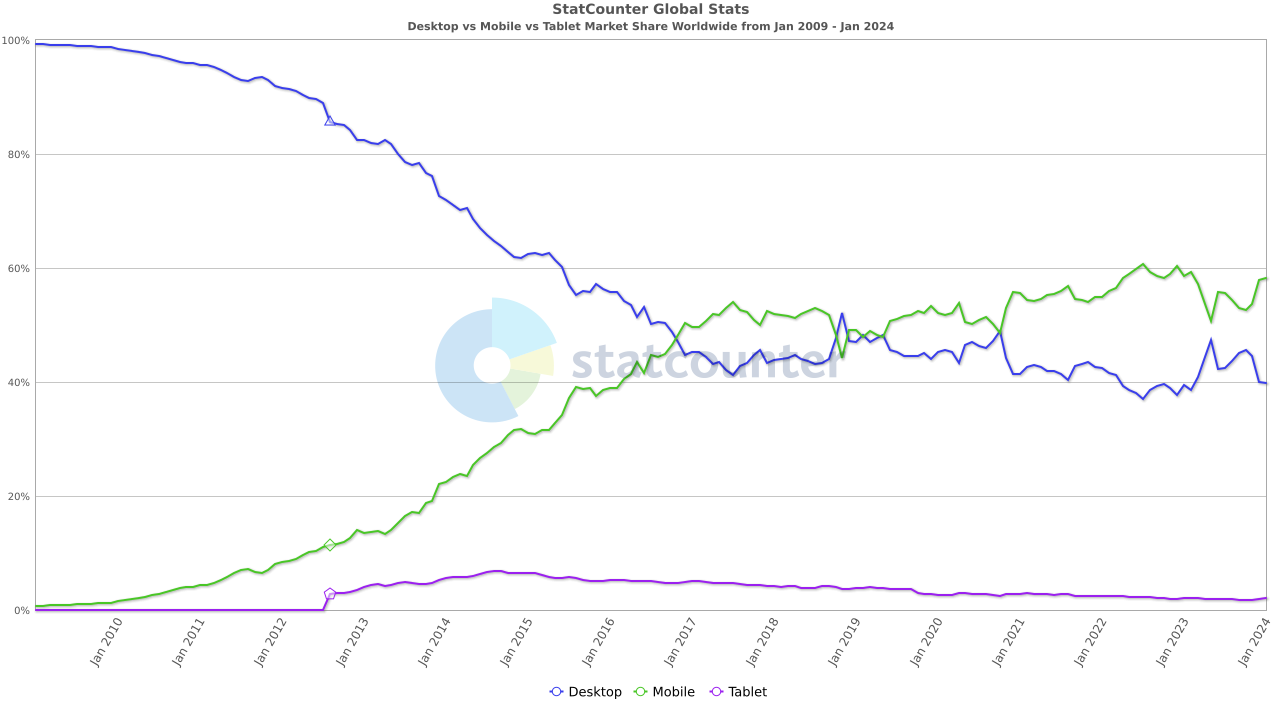
\includegraphics[width=\textwidth]{./figures/ch2_desktop-vs-mobile.png}
    \caption{Market shares of desktop, mobile and tablet devices, from January 2009 to January 2024 \cite{StatCountDMT}. Starting August 1st 2012, the chart counts tablets as a separate metric.}
    \label{FigStatCounterDMT}
\end{figure}

The trend of owning a mobile device shows that people prefer carrying a small and capable device around, rather than only being able to connect to the Internet using their fixed and comparatively large desktop device.

\section{Design differences and similarities between desktop and mobile}

\subsection{Evolution of desktop devices}

It is worth noticing that these two platforms could not be more similar to one another, yet have so many differences. Desktop devices have a notably different evolutionary tree to mobile devices, which means that not only do their shapes and buttons differ, but also their design philosophies.

Computers in their earliest forms were generally thought of as "boiler-room infrastructure" rather than personal devices. The advent of devices like the Apple II and software like VisiCalc, which was an advanced-for-the-time spreadsheet processor released in 1979, started to prove to the world that computers are not only useful when used by a trained team of experts, but can automatize tasks in the reach of a single employee \cite{NYBirthPC}.

These flashy, almost magical machines were starting to be capable of doing various tasks, from boring data processing to running graphics and games. This, combined with how they started to become more and more affordable, resulted in a boom in personal computer ownership starting in the 1980s.

\begin{figure}[htbp]
    \centering
    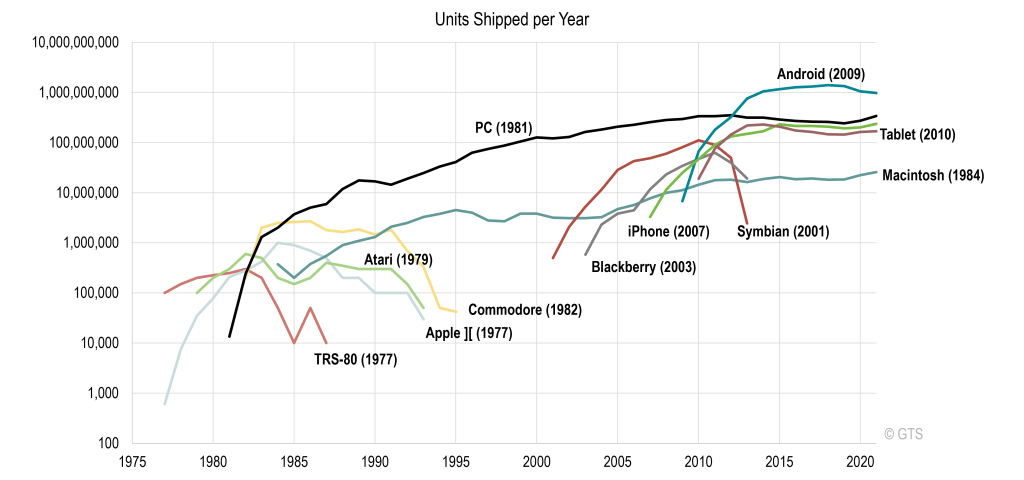
\includegraphics[width=\textwidth]{./figures/ch2_historical_pc_usage.png}
    \caption{Units Shipped per year for various desktop PCs and mobile devices, from 1977 to 2021 \cite{TGPCHis}.}
    \label{FigHistoricalPC}
\end{figure}

This direct lineage between the personal computer and pre-1970 mainframes is apparent in the architectures of common operating systems like Windows or Unix. Given how specialized machines, that required trained people to use, started to spread to less technically advanced end-users, it is understandable that computer and operating system vendors tried to simplify how their systems were used.

In particular, the Personal Computer (PC) developed by IBM has seen the longest lifetime of a single lineage of computers (Figure \ref{FigHistoricalPC}), being traceable all the way from 1981 to today. This shows that the evolution of the IBM PC occurred in incremental steps, and to avoid having software vendors be forced to upgrade their software upon release of every version, it is understandable that IBM offered a degree of backwards compatibility.

As a result, design decisions that made sense in the 1980s started to be less useful. A notable example of such design decisions can be found in modern Windows operating systems. The Microsoft documentation \cite{MSDNFolderNaming} has a clause that specifies a number of disallowed directory and file names, the likes of "CON", "PRN", "NUL", "AUX", and others, in addition to any combination of these names with any extension. This is very likely a result of the desire to keep backwards compatibility with old MS-DOS systems, that Windows can be directly traced to, which used these names as aliases for device drivers \cite{HusseinDeviceDrivers}.

\subsection{Evolution of mobile devices}
In comparison, the evolution of mobile devices and smartphones is very distinct and contained in a much shorter period of time.

The first device that was described as "the first time someone created a computer into the shape of a phone" is credited to be the IBM Simon, released around 1992. Boasting a touch screen and being portable, it had features such as a calculator and email. It has been described, retroactively, as "[being] the first smartphone. Twenty years ago, it envisioned our app-happy mobile lives, squeezing the features of a cell phone, pager, fax machine, and computer into an 18-ounce black brick"
\cite{SagerIraHistoryOfPhones}.

The year 1992 is very recent, compared to when the first computers started to become mainstream. This allowed phone manufacturers and OS vendors to learn from the mistakes done by personal computers, or optimize certain user experience facets.

An important step in the evolution of mobile devices is widely regarded as being the first iPhone. The hype Apple created about their new and flashy smartphone, culminating in around 11.000 print articles and 69 million hits on Google, seems to have been justified, and the phone was revolutionary, although somewhat flawed \cite{NYTAppleIPhoneRelease}. The iPhone defined a new era of smartphones, and many phone manufacturers have followed in the path that Apple laid out.

One of the core ideals of the iPhone is the ease of use. People that are non-technical find the iPhone accessible, and the way it seamlessly integrates with other Apple (sadly, only Apple) products proves that technology does not necessarily have to be hard to use \cite{SlashGearIPhoneOverAndroid}.

This trend manifests itself across the entire range of available mobile devices versus personal computers. Mobile phones are more widespread and are generally easier to use, having more friendly user interfaces and abstracting away hard technical details as much as possible.

\section{Native applications}

Mobile devices present ways of installing additional programs called "applications" that can extend the functionality of the device. Applications have proven to be the de-facto standard for implementing mobile functionality, and an ever-increasing number of companies offer their services through the apps that they constantly ask consumers to install.

From an architectural standpoint, these applications are strongly tied to the operating system architecture, and are therefore not portable.

\subsection{Architecture incompatibilities}

Having said that, an attempt at portability and standardization across mobile devices can be found within the Android Open Source Project (AOSP). An initiative by Google, the project offers a full mobile operating system under an open-source license, thus allowing any phone maker across the world to use it as a starting point for their own operating system.

While the AOSP initiative was a success and today many mobile devices have their roots in Android, phone manufacturers took to their own in creating an operating system with their own modifications, which make the Android ecosystem somewhat incompatible with itself, and lead to fragmentation of the Android market.

\begin{figure}[htbp]
    \centering
    \begin{subfigure}{.5\textwidth}
        \centering
        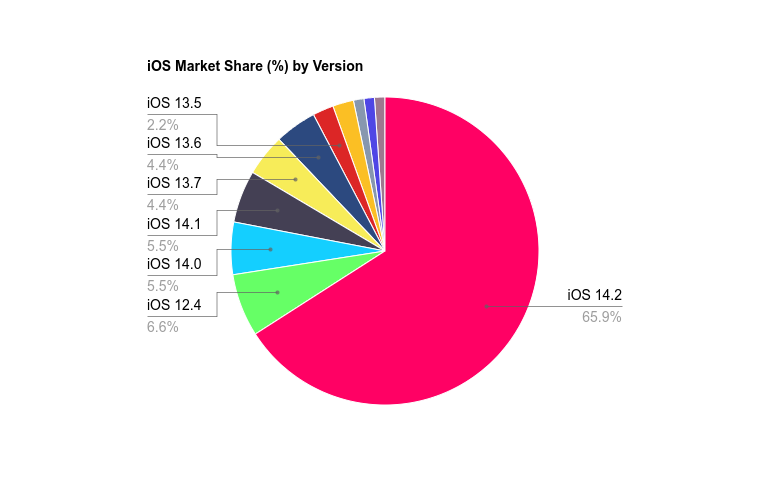
\includegraphics[width=\textwidth]{./figures/ch2_ios-market-share.png}
        \caption{iOS Market Share (\%)}
        \label{fig:sub1}
    \end{subfigure}%
    \begin{subfigure}{.5\textwidth}
        \centering
        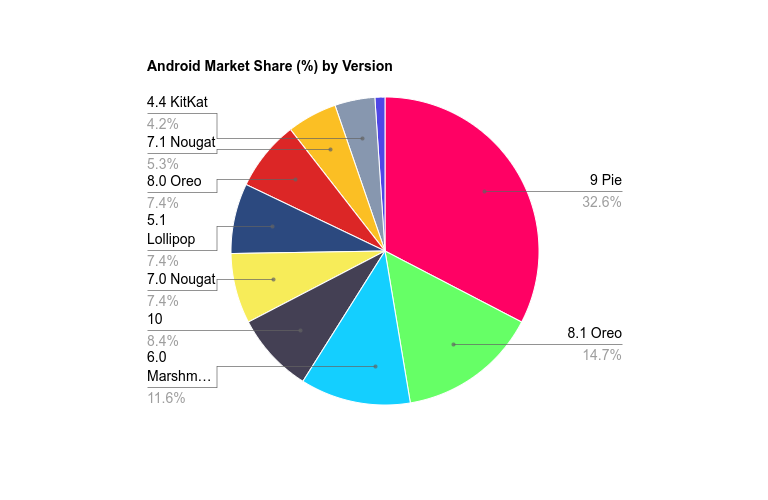
\includegraphics[width=\textwidth]{./figures/ch2_android-market-share.png}
        \caption{Android Market Share (\%)}
        \label{fig:sub2}
    \end{subfigure}
    \caption{Global market share of iOS versions, compared to Android versions \cite{StatCounterIOSVersionsMarketShare} \cite{XDADevsAndroidVersionsMarketShare}.}
    \label{FigAndroidVsIosFragmentation}
\end{figure}

A comparison between the Android and iOS ecosystems, with the former based on the AOSP project and the latter a proprietary system owned by Apple, presented in figure \ref{FigAndroidVsIosFragmentation}, shows the striking difference between the market shares of the respective latest versions. The Android market fragmentation can be attributed indirectly to its open-source model, and is in direct contrast with the proprietary model of Apple and its control over the entire iOS ecosystem.

This is but one example of the incompatibilities of native application across mobile device operating systems. Generally, developing an application that is desired to reach as many users as possible requires developing for a range of architectures, such as iOS, Android or Huawei.

\subsection{Ecosystem control}
Distribution of native applications is generally done using application marketplaces that are proprietary to each phone manufacturer. Examples of such marketplaces include Google's Play Store, Apple's App Store, or Huawei's AppGallery. These marketplaces provide services such as automatic updates and ability to review apps.

However, these marketplaces also represent a way of controlling the application ecosystem. One marketplace known for very carefully curating apps in its distribution system is Apple's App Store.

Apple imposes very strict rules on its applications, aiming to preserve their users' privacy and experience. As an example, they restrict access to device sensors that can be used for user fingerprinting, and require justification if a sensor is requested by an application \cite{ZdnetNewAppleStoreRules}.

This being said however, it is also worth mentioning that Apple takes a commission of all sales performed through its App Store (store purchases, in-app purchases) that can reach percents of 30\%. These high profits have the potential to justify some other market manipulation tactics that Apple employs.

Apple is known to handle Internet browsing on iOS in ways that can be considered a way of market manipulation. Instead of offering alternatives to their high-commission marketplace, they intentionally avoid implementing important Web APIs in their proprietary WebKit browser engine used by Safari \cite{ZdnetAppleDeclinedWebApis}, while not allowing, as per App Store policy, alternative browser engines \cite{AppleGuidelinesWebkit} (note that regulations in the European Union might force Apple to provide limited support for such alternatives \cite{AppleAlternativeBrowsersEU}).

Apple's reasoning for not implementing Web APIs relating to phone sensors and telemetry (NFC, battery, bluetooth, geo-location) is that they value users' privacy, even though these APIs are not that related to privacy but rather to an application's ability to get shipped as a Web app rather than a native, App Store app.

\subsection{Device access}
By nature of being specifically built for the target architecture, native applications have an unmatched capability of making use of the phone hardware. Having no additional layers between application code and operating system (e.g. a browser runtime and sandbox), native code has access to all the operating system system calls exposed to native applications, and can also achieve unmatched runtime performance.

% \section{Hybrid (cross-platform interpreted) applications}

\section{Web applications}
Even in the early days of the Internet, rudimentary forms of websites, that can be called web applications, existed. One of the pioneering frameworks for creating such interactive experiences begun as the Personal Home Page programming language, also known as PHP, released around 1995. It had the ability to render dynamic pages and handle user forms, which already compose a functional web application. Over the years, PHP has grown in popularity and it has got incremental updates, such that it now powers over 70\% of the websites on the Internet \cite{TurnkeyPHPIsNotDead}. It envisioned having web applications work in a simple "request page $\rightarrow$ response with page" model (figure \ref{FigPHPSeqDiag}).

\begin{figure}[htbp]
    \centering
    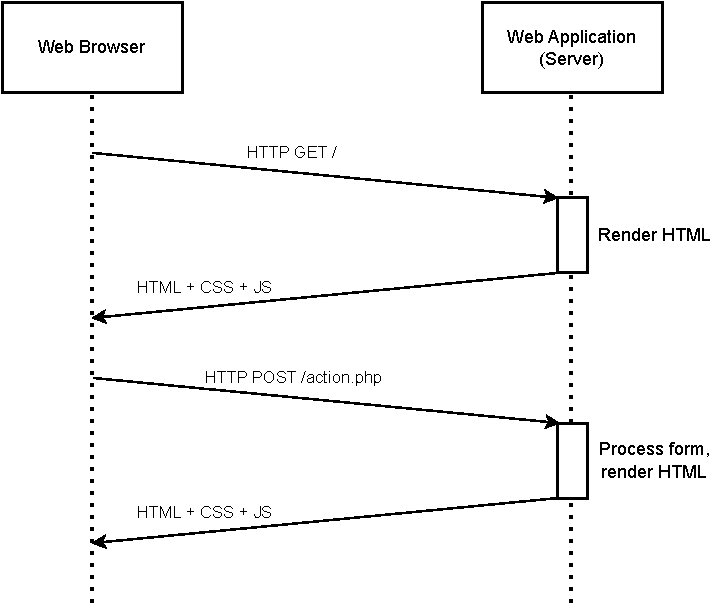
\includegraphics[width=0.7\textwidth]{./figures/ch2_php-seq-diag.pdf}
    \caption{Illustrative diagram of how a PHP-based website might process requests.}
    \label{FigPHPSeqDiag}
\end{figure}

An important step in the evolution of dynamic web pages was the introduction of AJAX around the year 2005 \cite{PWAShortHist}. AJAX, short for Asynchronous JavaScript and XML, enabled web pages to make additional HTTP requests initiated by client-side JavaScript code. These asynchronous HTTP requests could then be used to dynamically update contents of the page, without needing a full page refresh (figure \ref{FigAJAXSeqDiag}). However, a backend server that can generate HTML code was needed to render the initial page, even if subsequent AJAX requests didn't transfer information in HTML representation (ie. JSON).

\begin{figure}[htbp]
    \centering
    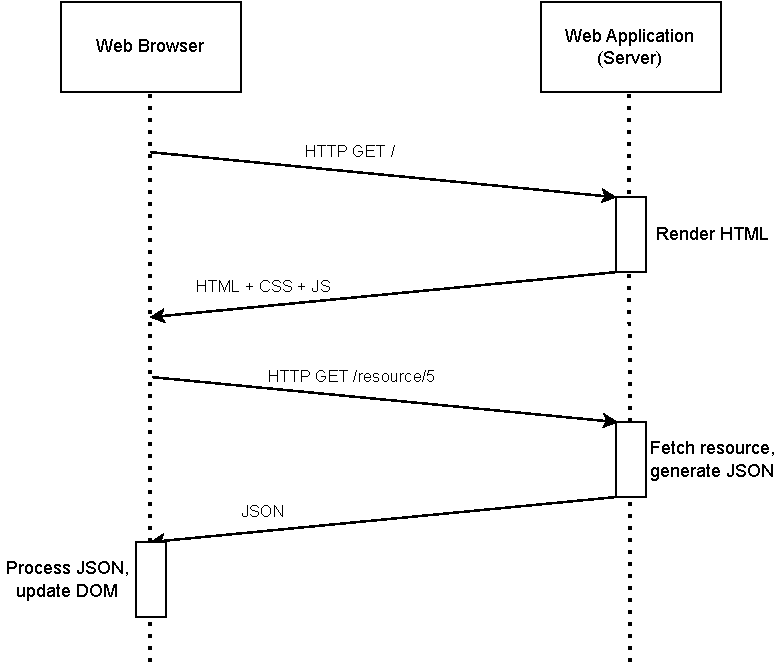
\includegraphics[width=0.7\textwidth]{./figures/ch2_ajax-seq-diag.pdf}
    \caption{Illustrative diagram of how a website making use of AJAX calls might process requests.}
    \label{FigAJAXSeqDiag}
\end{figure}

Incremental improvements in the JavaScript standards, and new and novel frontend frameworks that attempted to ease the injection of \( f(state) \Rightarrow view \) (such as React, Angular) enabled a new form of web application to take shape: that of the Single Page Application.

The Single Page Application enabled separating an application into two completely separate components: a backend and a frontend. For the first time, backends could expose some endpoints, collectively called an API, that then the frontend could use to communicate with the backend (figure \ref{FigSPASeqDiag}). This separation enabled the frontend to be easily shipped as a static site across the world, the backend to become extremely simple and only communicate using JSON/XML, and so much more.

\begin{figure}[htbp]
    \centering
    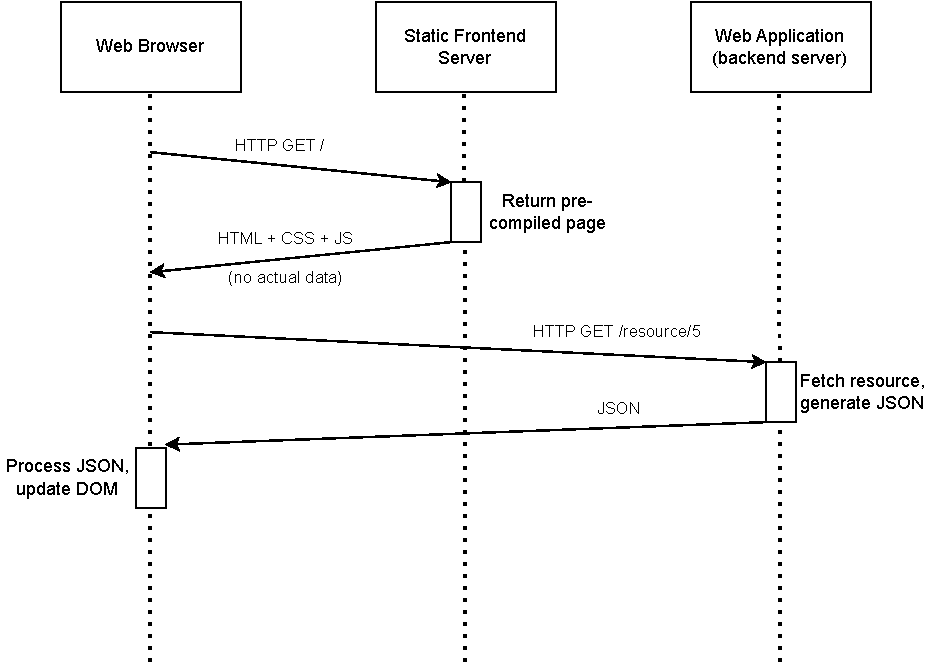
\includegraphics[width=0.85\textwidth]{./figures/ch2_spa-seq-diag.pdf}
    \caption{Illustrative diagram of how an application with separate backend and frontend might process requests.}
    \label{FigSPASeqDiag}
\end{figure}

\subsection{Browser inconsistencies}

Although in a much better state nowadays, browsers often preferentially implement certain Web APIs, creating many subtle incompatibilities between browser vendors. Tools like "Can I use" \cite{CanIUse} are the first thing a web developer checks for whenever they want to use a more obscure Web API.

However, API and engine differences have historically been mitigated by use of polyfills. Tools like Babel or TypeScript can also aid by providing a build step to JavaScript code that can transform the code to automatically enable support for various JavaScript standards.

Additionally, minor visual inconsistencies can also occur within the same brow\-ser vendor. Users might have different font sets installed, different screen sizes, or use browser functionalities that alter the page, like zoom, reader mode, etc.

\subsection{Browser sandbox}
All web applications that run in a browser are subject to the sandbox that the brow\-ser confines the JavaScript code within. Web applications can only access device capabilities that the browser provides access through, and can only do so reliably if they are covered by a standardized Web API.

This can understandably apply limitations to what an application shipped using the Web can do.

\subsection{Decentralized distribution}
Web applications are always distributed to users by means of the Internet. This means that there exists no single authority that can veto the distribution of certain applications, unlike the mobile marketplaces mentioned above.

Additionally, by nature, web applications are always kept up-to-date. They are downloaded on-demand, meaning that updates can be transparently and easily pushed to users. Even if the frontend is cached on the end-users' devices, the developers can be sure that setting a certain cache validity period means that no user will have the old version of the app once that validity period expires.

\subsection{The step towards PWA}

It is worth noticing that the "static frontend" component shown in figure \ref{FigSPASeqDiag} can be treated in a language-agnostic way. The frontend can easily be written using any frameworks or languages of preference (React, Angular, Vue; JavaScript, PyScript, compiled WebAssembly), without needing to alter in any way the backend infrastructure. In fact, we need not be constrained by something that can run in a browser: this frontend can even take the form of a mobile application.

We have already examined mobile applications, so it is time to explore a way to bring out the best of both worlds, using Progressive Web Apps.

\section{Progressive Web Apps}
